\newif\ifccs
\ccsfalse

\ifccs
\input{preamble_ccs.tex}
\else
%%%%%%%%%%%%%%%%%%%%%%
%usenix
%\documentclass[letterpaper,twocolumn,10pt]{article}
%\usepackage{usenix2019,epsfig,endnotes}
%%%%%%%%%%%%%%%%%%%%%%
%CCS
%\documentclass[sigconf, anonymous]{acmart}

% remove reference format for submission
%\settopmatter{printacmref=false}

% remove copyright box for submission
%\renewcommand\footnotetextcopyrightpermission[1]{}

% control headers 
%\fancyhf{} 
%\fancyhead[C]{Anonymous submission \#9999 to ACM CCS 2019} % TODO: replace 9999 with your paper number
%\fancyfoot[C]{\thepage}

%\setcopyright{none} % No copyright notice required for submissions
%\acmConference[Anonymous Submission to ACM CCS 2019]{ACM Conference on Computer and Communications Security}{Due 5 February 2019}{London, UK}
%\acmYear{2019}

%%%%%%%%%%%%%%%%%%%%%%

%S&P
\documentclass[conference]{IEEEtran}

\newif\ifdraft
%\drafttrue

\usepackage{xcolor}
\usepackage{graphicx,pifont}
\usepackage{adjustbox}
\usepackage{caption}
\usepackage{subcaption}
\usepackage{mathtools}
\usepackage{mathrsfs}
\usepackage{xspace}
\usepackage{url}
\usepackage{pifont}
\usepackage{listings}
\usepackage{multirow}
\usepackage{wasysym}
\usepackage{array}

%\usepackage[font={small}]{caption}
%\usepackage{enumitem}
\usepackage{cite}
%\usepackage{flushend}
\usepackage{hyperref}
%\usepackage{caption}



%% Compacting 
%%
%\usepackage[
%all=normal,floats=tight
%,paragraphs=tight
%,wordspacing=tight
%,mathspacing=tight
%,mathdisplays=tight
%]{savetrees}
%\usepackage[compact]{titlesec}


\lstset{
  basicstyle=\ttfamily,
  numbers=left, xleftmargin=2em,frame=single,framexleftmargin=1.5em,
  %numberstyle=\tiny,
  columns=fullflexible,
  showstringspaces=false,
  commentstyle=\color{gray}\upshape
}

\lstdefinelanguage{HTML}
{
  morestring=[b]",
  morestring=[s]{>}{<},
  morecomment=[s]{<?}{?>},
  stringstyle=\color{black},
  identifierstyle=\color{darkblue},
  keywordstyle=\color{blue},
  morekeywords={form,input,encrypted,Input}
}

\colorlet{punct}{red!70!black}
\definecolor{background}{HTML}{EEEEEE}
\definecolor{delim}{RGB}{20,105,176}
\colorlet{numb}{magenta!20!black}

\lstdefinelanguage{json}{
    basicstyle=\small\ttfamily,
    numbers=left,
    numberstyle=\scriptsize,
    stepnumber=1,
    numbersep=8pt,
    showstringspaces=false,
    breaklines=true,
    frame=lines,
    backgroundcolor=\color{background},
    morekeywords={formId, formName, ui, id, type, label, text, trigger, domain},
    literate=
     *{0}{{{\color{numb}0}}}{1}
      {1}{{{\color{numb}1}}}{1}
      {2}{{{\color{numb}2}}}{1}
      {3}{{{\color{numb}3}}}{1}
      {4}{{{\color{numb}4}}}{1}
      {5}{{{\color{numb}5}}}{1}
      {6}{{{\color{numb}6}}}{1}
      {7}{{{\color{numb}7}}}{1}
      {8}{{{\color{numb}8}}}{1}
      {9}{{{\color{numb}9}}}{1}
      {:}{{{\color{punct}{:}}}}{1}
      {,}{{{\color{punct}{,}}}}{1}
      {\{}{{{\color{delim}{\{}}}}{1}
      {\}}{{{\color{delim}{\}}}}}{1}
      {[}{{{\color{delim}{[}}}}{1}
      {]}{{{\color{delim}{]}}}}{1},
}

\renewcommand\lstlistingname{Specification}

\let\oldding\ding% Store old \ding in \oldding
\renewcommand{\ding}[2][1]{\scalebox{#1}{\oldding{#2}}}% Scale \oldding via optional argument

\newcommand{\zero}{\ding[1.2]{171}\xspace}
\newcommand{\one}{\ding[1.2]{172}\xspace}
\newcommand{\two}{\ding[1.2]{173}\xspace}
\newcommand{\three}{\ding[1.2]{174}\xspace}
\newcommand{\four}{\ding[1.2]{175}\xspace}
\newcommand{\five}{\ding[1.2]{176}\xspace}
\newcommand{\six}{\ding[1.2]{177}\xspace}
\newcommand{\seven}{\ding[1.2]{178}\xspace}
\newcommand{\eight}{\ding[1.2]{179}\xspace}
\newcommand{\nine}{\ding[1.2]{180}\xspace}
\newcommand{\ten}{\ding[1.2]{181}\xspace}

\usepackage{color, colortbl}
\definecolor{gray}{rgb}{0.4,0.4,0.4}
\definecolor{darkblue}{rgb}{0.0,0.0,0.6}
\definecolor{cyan}{rgb}{0.0,0.6,0.6}
%\definecolor{Gray}{gray}{0.1}

\definecolor{Gray}{rgb}{0.88, 0.88, 0.88}
\definecolor{HGray}{rgb}{0.7, 0.7, 0.7}
%\definecolor{HGray}{gray}{0.8}

\newcommand{\yes}{\CIRCLE} 
\newcommand{\no}{\Circle} 
\newcommand{\yesNope}{\LEFTcircle} 


\newcommand{\red}[1]{\textcolor{red}{#1}} 

\newcommand{\ad}[1]{\textcolor{red}{Aritra: #1}}
\newcommand{\srdjan}[1]{\textcolor{brown}{Srdjan: #1}}
\newcommand{\todo}[1]{\textcolor{red}{TODO: #1}}
\newcommand{\tocite}{\textcolor{blue}{[cite]}}

%\widowpenalty 200000
%\clubpenalty 200000
%\usepackage[compact]{titlesec}

\newcommand{\name}{\textsc{GuardIOn}\xspace}
\newcommand{\tool}{\name}
\newcommand{\device}{\textsc{Bridge}\xspace}
\newcommand{\pop}{proof-of-pointer\xspace}
\newcommand{\Pop}{Proof-of-pointer\xspace}

\newcommand{\poa}{proof-of-action\xspace}
\newcommand{\Poa}{Proof-of-action\xspace}

\newcommand{\poui}{proof-of-UI\xspace}
\newcommand{\Poui}{Proof-of-UI\xspace}
\newcommand{\server}{\textsc{Server}\xspace}

\newcommand{\toolname}{\name\xspace}

\newcommand{\usb}{USB\xspace}
\newcommand{\bluetooth}{Bluetooth\xspace}
\newcommand{\webusb}{WebUSB\xspace}
\newcommand{\html}{HTML\xspace}
\newcommand{\webbt}{WebBluetooth\xspace}
\newcommand{\http}{HTTP\xspace}
\newcommand{\https}{HTTPS\xspace}
\newcommand{\tls}{TLS\xspace}
\newcommand{\ssl}{\texttt{SSl}\xspace}
\newcommand{\onSelect}{\texttt{onSelect()}\xspace}

%\newcommand{\myparagraph}[1]{{\scshape \bfseries #1.}}
\newcommand{\myparagraph}[1]{\textbf{#1.}}

\newcommand{\webrtc}{\texttt{WebRTC}\xspace}
\newcommand{\js}{JavaScript\xspace}

\newcommand{\mytab}{~~~}
\newcommand{\java}{\textsc{Java}\xspace}

\definecolor{Gray}{gray}{0.85}
\definecolor{LightCyan}{rgb}{0.88,1,1}

\newcommand\MyLBrace[2]{%
  \left.\rule{0pt}{#1}\right\}\text{#2}}



\DeclareGraphicsExtensions{.pdf,.jpeg,.png,.jpg}


%------------------------------------------------------------------------------
%                                Space savers.
%------------------------------------------------------------------------------

% This mylist environment indents items, and saves less space than the above.
\newcounter{myctr}
\newenvironment{mylist}{\begin{list}{(\textbf{\roman{myctr}})}
{\usecounter{myctr}
\setlength{\topsep}{1mm}\setlength{\itemsep}{0.5mm}
\setlength{\parsep}{0.5mm}
\setlength{\itemindent}{1mm}\setlength{\partopsep}{0mm}
\setlength{\labelwidth}{-2mm}
\setlength{\leftmargin}{1mm}}}{\end{list}}

% Space saving List environment for itemizing.
\newenvironment{mybullet}{\begin{list}{$\bullet$}
{\setlength{\topsep}{1mm}\setlength{\itemsep}{0.5mm}
\setlength{\parsep}{0.5mm}
\setlength{\itemindent}{0mm}\setlength{\partopsep}{0mm}
\setlength{\labelwidth}{-2mm}
\setlength{\leftmargin}{0mm}}}{\end{list}}

\fi



\newif\ifdesperatetime
%\desperatetimetrue

\graphicspath{{images/}}

\begin{document}

\author{
    \IEEEauthorblockN{Aritra Dhar}
    \IEEEauthorblockA{ETH Zurich}
    \and
    \IEEEauthorblockN{Enis Ulqinaku}
    \IEEEauthorblockA{ETH Zurich}
    \and
    \IEEEauthorblockN{Kari Kostiainen}
    \IEEEauthorblockA{ETH Zurich}
    \and
    \IEEEauthorblockN{Srdjan Capkun}
    \IEEEauthorblockA{ETH Zurich}
}

\title{\name: Root-of-Trust for IO \\ in Compromised Platforms}

\ifccs
\else
\maketitle
\fi

\thispagestyle{plain}
\pagestyle{plain}

\begin{abstract}
 

\emph{Security} and \emph{safety-critical} remote applications such as e-voting, online banking, industrial control systems, medical devices, and home automation systems rely upon user interaction that is typically performed through web applications. Trusted path to such remote systems is critical in the presence of an attacker that controls the computer that the user operates. Such a powerful attacker can observe and modify any IO data without being detected by the user or the server. We investigate the security of previous research proposals that address this problem and observe several drawbacks that make them vulnerable to advance UI manipulation attacks.Based on these observations we define a novel set of requirements for secure IO operation in the presence of a compromised host.
  
We propose \name, a system that ensures the integrity and confidentiality of the user's IO employing a trusted low-TCB device that sits between the attacker-controlled host and the IO devices. Therefore, \name device can intercept the display signal and user inputs from the keyboard and mouse. Furthermore, it can overlay secure UI on top of the HDMI frames generated by the untrusted host. \name integrates well in the existing infrastructure, it requires small changes in the server-side, works with any browser without installing any additional software, and does not change significantly the user experience. Finally, we implement a prototype of \name which is a plug-and-play device and evaluate its performance.


\end{abstract}


\ifccs
\maketitle
\else
\fi

\section{Introduction}
\label{sec:intro}



\red{First draft of the intro. Flow: motivation and examples -> related works -> our approach -> contributions}

\begin{figure}[t]
\centering
\includegraphics[trim={0 1cm 10cm 0}, clip, width=\linewidth]{motivation.pdf}
\caption{\textbf{Motivating examples.} 1) Pointer based UI elements that sets parameters to remote safety-critical device, 2) E-voting where the voting privacy and integrity is critical, 3) Financial transactions such as bitcoin wallet that shows sensitive information such as the user's private key and 4) web applications that provide an option for the user to reveal credentials.}
\spacesave
\label{fig:motivation}
\centering
\end{figure}


Human interaction with computers is one of the most fundamental components in today's complex systems, and interfaces are crucial for the interactions. All computing devices, such as desktop computers, smartwatches, embedded devices provide some input mechanisms via the user interfaces (UI) where the users can provide input to the computers. These input interfaces are the embodiments of the human-computer interaction (HCI). Critical infrastructures and automation systems rely on human input, and the correctness of the input is of uttermost importance. Human interaction with the computer systems over the last few decades evolves both in diversity and complexity. This gives rise to a major threat concerning the integrity and the confidentiality of the user input. Recent revelations like Snowden leaks show that powerful attackers such as state nations can compromise general purpose computing systems (we call them \emph{host} systems, e.g., computers, smartphone, etc.) that include both operating systems and hardware. Research works such as A2~\cite{A2} shows the first fabrication-time attack that can leverage the space common to Application-Specific Integrated Circuit (ASIC) layouts to implement malicious circuits. Such attacks are major threats to the security and privacy of the user interaction with the system as the attacker can monitor and manipulate user interactions. 
Figure~\ref{fig:motivation} provides four such potential uses cases out of many, where the integrity and confidentiality of user IO data are critical. Networked safety-critical systems, such as Programmable Logic Controllers in a factory plant, are often remotely configurable by administrators through web-based interfaces. Other applications such as home automation systems, medical devices also expose their functionality through web APIs. Apart from the cyber-physical system, other web-based applications such as internet banking, user input are very critical. Manipulating user input in these applications could lead to catastrophic failures, even compromise the safety of humans. Hence, integrity is one of the major aspects while providing input parameters to a critical system. Apart from the integrity, the confidentiality of the user input is also of utmost importance for applications like e-voting, online messenger, web-service credentials, bitcoin wallet, etc. Secure transport layer protocols such as \https (or \tls) can be employed to secure the communication between the host system and the remote server, but the protocols assume that the host system is trusted which may not be the case provided the aforementioned attacker model.

InContext~\cite{huang2012clickjacking} presents different clickjacking attacks variants and their solution by ensuring context (both temporal and visual) and pointer integrity in the trusted browser setting. Trusted hypervisors and secure micro-kernels are also choices for contrasting Trusted path. Sel4~\cite{klein2009sel4} is a functional hypervisor that is formally verified and has a kernel size of only $8400$ lines of code. In work done by Zhou et al.~\cite{zhou2012building}, the authors proposed a generic trusted path on $x86$ systems in pure hypervisor-based design. Examples of other hypervisor-based works can be found in systems such as Overshadow~\cite{Overshadow}, Virtual ghost~\cite{criswell2014virtual}, Inktag~\cite{hofmann2013inktag}, TrustVisor~\cite{mccune2010trustvisor}, Splitting interfaces~\cite{ta2006splitting}, $SP^3$~\cite{yang2008using}, etc.



There exist several research works that looked into the security of user IO data. \emph{Trusted path} is the concept that in-theory solves the problem of user IO security between the user and the end-system. The trusted path provides a secure channel between the user (HID) to the end system, and this end system could be a remote server or a local computer. Several ways could be employed to realize the trusted path. For example, Filyanov et. al~\cite{filyanov2011uni} proposed transaction confirmation device that requires the user to use a separate device to confirm the input parameters. This allows the user to review her input data on a separate trusted device that is physically separated from the untrusted host. Trusted execution environments (TEE) such as Intel SGX, ARM TrustZone, TPM, Intel TXT, etc. provide isolated code execution, and can be used to achieve trusted path. Previous research works such as Intel SGX and trusted hypervisor-based SGXIO~\cite{weiser2017sgxio}, Intel SGX based ProximiTEE~\cite{dhar2018proximitee}, TPM and TXT based trusted path~\cite{filyanov2011uni}, and ARM TrustZone based trusted path~\cite{filyanov2011uni,sun2015trustotp} are the example of trusted path construction based on TEEs. All of these solutions require specialized platforms with processors that support such infrastructure. VButton~\cite{li2018vbutton} uses ARM TrustZone to overlay buttons on the mobile devices that confirm if the user taps on a specific button. Processor-TEE such as Intel SGX primarily provides execution privacy and code integrity. In most of the cases, IO is still mediated by the OS. 


\myparagraph{Our approach} In this paper, we present our solution \name, that leverage the concept of bump-in-the-wire~\cite{McCPerRei2006} to establish a trusted path between a remote server and user IO devices. \name uses a low-TCB auxiliary device that works a generic IO hub between all user IO devices and the untrusted host. 
We assume that the host and the network are attacker-controlled. The trusted components include the remote server, \device, and IO devices. \device intercepts the display signal from the host, analyze them to understand the correct user context, such as if the user moved her mouse over a specific UI element and click there. The \device also intercepts the mouse and keyboard signal and match them with the display signal that is received from the untrusted host. If both the input and output co-relates, the \device signs all the input and send them to the remote server. \device does not have any explicit network capability to communicate with the remote server. Instead, the \device uses the host as an untrusted transport.

\myparagraph{Contribution} Here we provide the major contributions of this paper:
\begin{mylist}
  \item
\end{mylist}

\myparagraph{Organization of the paper}
\section{Background: Secure Web UI}
\label{sec:background}


\section{Problem Statement}
\label{sec:problemStatement}

\begin{figure}[t]
\centering
%\includegraphics[trim={0 14cm 17cm 0}, clip, width=0.9\linewidth]{systemModel.pdf}
\includegraphics[trim={0 14cm 17cm 0}, clip, width=0.9\linewidth]{systemModel_all.pdf}
\caption{\textbf{Trusted path system model.} The figures shows the system and the attacker model of the trusted path. We generally consider two trusted path scenarios, \one trusted path to a remote server, and \two trusted path to a trusted execution environment (TEE) such as the Intel SGX.}
\label{fig:systemModel}
\centering
\end{figure}


In this section, we motivate our work, explain the security properties, describe existing literature lacks proper solution and explain the goals of our work.



\begin{figure}[t]
\footnotesize
    \centering
    \begin{tikzpicture}[
solved/.style={rectangle,draw,fill=purple!40, rounded corners, align=center},
not/.style={rectangle, draw,fill=orange!60, rounded corners, align=center},
neutral/.style={rectangle, draw, rounded corners, align=center, fill=black!5}
]]
    \node[neutral](root) {Trusted path}
    child { node[neutral, yshift=12pt] (hw) {External\\ HW}}
    child { node[neutral, yshift=8pt, xshift=10pt] (tc) {Transaction\\ confirmation\\ Device}}  
    child { node[neutral, yshift=12pt, xshift=20pt] (tee) {TEE}
      child { node[neutral, yshift=0pt, xshift=-5pt] (teehv) {Hypervisor+\\TEE}}
      child { node[neutral, yshift=0pt, xshift=2pt] (teehw) {TEE + \\ External HW} } }
      child { node[neutral, yshift=8pt, xshift=15pt] (br) {Browser\\ Based}}   
     child { node[neutral, yshift=12pt, xshift=20pt] (hv) {Hypervisor}}  ;
    
      

    \node[below=0cm of hw] {\textbf{\name}};
    \node[below=0cm of tc] {Uni-dir~\cite{filyanov2011uni}};
    \node[below=0cm of hv] {Overshadow~\cite{Overshadow}};
    \node[below=0cm of teehv] {SGXIO~\cite{weiser2017sgxio}};
    \node[below=0cm of teehw] {Fidelius~\cite{Fidelius}};
     \node[below=0cm of br] {InContext~\cite{blake1998authenticated}};

    
    \end{tikzpicture}
    
   \caption{\textbf{Summarization of existing trusted path solutions} by their trust assumptions. A detailed description of the related works is discussed in Table~\ref{tab:relatedWorks}.}
     \label{fig:relatedWorksTree}
\end{figure}


\subsection{Motivation: IO for Remote Data and Safety-critical System}


A user communicates with a remote server through a host system, which gives the host access to the plaintext data that goes from the user to the server and vice-versa. Thus, a compromised host can always observe or modify the information exchanged between the user and the server. An adversary that compromises the user's host can alter user intentions, i.e., it can perform arbitrary actions on behalf of the user. Such an adversary is very powerful and difficult to detect or prevent by the remote server. The consequences of such attacks might be severe when safety-critical applications are targeted. The attacker can pass the wrong input to a remote safety-critical system such as a medical device, power plant, etc. 

Trusted execution environments (TEEs) such as Intel SGX enable remote trust into the code executing on the processor, effectively eliminating the need to trust more significant code base (motherboard, memory modules, OS and other applications). However, despite the TEEs, the problem of isolating user's input and output remains as the operating system handles the IO drivers and data. Therefore, service providers typically operate with the assumption that honest users genuinely generate the data they receive and not altered by a compromised computer. In a few use cases, e.g., online payments, the service providers ask for user confirmation on a second device (phone or specialized hardware) to detect such attacks. However, this solution is limited to applications in which a user can check the input on a secondary device. 

A \emph{Trusted path} provides confidentiality and integrity to the IO data exchanged between the users and the end systems. In principle, a trusted path solve the general security problem of the IO data. But practically establishing a trusted path in general IO devices is a nontrivial problem specifically if one considers the plethora of complex UI objects and input methods as well as different security and functional properties that a solution should satisfy.

\iffalse
\subsection{Security Properties}

A \emph{Trusted path} provides confidentiality and integrity to the IO data exchanged between the users and the end systems. In principle, a trusted path solve the general security problem of the IO data. But practically establishing a trusted path in general IO devices is a nontrivial problem specifically if one considers the plethora of complex UI objects and input methods as well as different security and functional properties that a solution should satisfy. We list these properties below. 


\begin{mylist}
  \item \textbf{Input integrity and privacy.} These properties define that any input that is coming from the user input devices are fully protected in two ways: i) the input issued by the user reaches to the remote end-point as it was generated by the user - \emph{integrity}, and ii) in specific application scenarios, the attacker-controlled host is entirely oblivious about the input from the user - \emph{confidentiality}. The trusted path system should consider a wide range of input devices, such as keyboard, mouse, touch etc. We consider any sort of input action by the user that may include moving the mouse or using the keyboard navigation keys to select a specific item in a list.
  
  
  \item \textbf{Output integrity and confidentiality.} Similar to the input integrity, output integrity ensures that information that is sent by the remote endpoint is presented to the user as it was meant to be. One example of output integrity is the integrity of the UI elements. Such property ensures that the host system renders the UI elements faithfully as they were sent by the remote system. Output confidentiality ensures that the information sent by the remote server can not be accessed by the attacker-controlled host. 
  
 %  \item \textbf{Usability.} The trusted path should neither change the typical user interaction with a computer nor should require extensive changes into the existing systems.

  As discussed on the Section~\ref{sec:securityAnalysis}, ensuring output integrity is essential for providing input integrity against advanced attackers that trick the user into sending non-legitimate data to the server. For example, the user wants to send a number \texttt{10} to the server, but the malicious host shows on screen \texttt{100} and fools the user into believing he mistyped a \texttt{0}. The user deletes one \texttt{0} and sees \texttt{10} on the screen---as he intended initially---and submits the data, however, on the server arrives just \texttt{1}. 
  
  Providing output integrity is a challenging task even on systems that have a trusted component that overlays parts of the HDMI frames generated by the untrusted host. Previous works~\cite{huang2012clickjacking} show that when a trusted component and an untrusted one share a screen, the attacker can still manipulate the user to commit unintentional actions to the trusted UI if the system is not designed properly. In our solution we want to guarantee that the user is aware of the UI elements (trusted or untrusted) that she interacts with, therefore preventing related attacks.
  \end{mylist}

\fi

\iffalse
\myparagraph{Advantages}

\begin{enumerate}
  \item The \device does not need to know the formatting/template of the page. As the \device only looks to the current mouse position, the structure of the page is somewhat irrelevant (?).
\end{enumerate}
\fi

\iffalse
\begin{table}[t]
\small
\centering
  \begin{tabular}{ l | c | c }
    \hline
     & TEE & no TEE \\ \hline
    \multirow{6}{*}{Hypervisor-based} & \multirow{6}{*}{SGX IO~\cite{weiser2017sgxio}} & Overshadow~\cite{Overshadow} \\ 
    & & Virtual ghost~\cite{criswell2014virtual}\\ 
    & & Inktag~\cite{hofmann2013inktag}\\ 
    & & TrustVisor~\cite{mccune2010trustvisor} \\ 
    & & Splitting interfaces~\cite{ta2006splitting}\\ 
    & & $SP^3$~\cite{yang2008using}\\ \hline
   Isolated execution & BASTION-SGX~\cite{BASTION-SGX} & Slice~\cite{azab2011sice}\\ 
   of APIs/Drivers & TrustOTP~\cite{sun2015trustotp} & CARMA~\cite{vasudevan2012carma} \\ \hline
   External trusted  &  \multirow{2}{*}{Fidelius~\cite{Fidelius}} & IntegriKey~\cite{IntegriKey} \\
   hardware based &  & FPGA-based~\cite{brandon2017trusted} \\
    %&  & \textcolor{blue}{Our Solution (I + O + Activity)} \\
    \hline
    Handles both & \multirow{2}{*}{\textcolor{red}{None}} & \multirow{2}{*}{\textcolor{blue}{Our Solution}} \\
    keyboard + mouse &  & \\
    \hline
  \end{tabular}
  \caption{Summarization of existing trusted path solutions. Note that in the table, switching systems from left to right or top to bottom, reduces the trust assumption. For example, TEE based solutions, such as SGX-based trusted path solution requires trust on the physical processor packages, SGX APIs, quoting and launch enclaves and Intel attestation service.}
\end{table}
\fi


\subsection{Existing Solutions and their drawbacks}

There exist several works that try to solve the problem of trusted paths for IO devices in the presence of a compromised host. But all of these solutions targeted for different problem settings and models. Figure~\ref{fig:relatedWorksTree} provides a board classification of the related works and illustrates where our proposed work stands concerning them. Detailed description of the related research is also described in Table~\ref{tab:relatedWorks} in Appendix~\ref{sec:summaryResearch}.

\subsubsection{Transaction confirmation devices} In their paper, Filyanov et. al~\cite{filyanov2011uni} proposed transaction confirmation device that requires the user to use a separate device to confirm the input parameters. The transaction confirmation suffers from two significant drawbacks. First, it introduces lots of cognitive load over the user and may force the user to confirm their action without even looking to the input data. This makes the transaction confirmation device unusable in day-to-day interactions. Second, transaction confirmation is not practical/suitable for complex interaction, rather simple text-based inputs. \name supports generic input devices and supports complex user interfaces and user interactions. Moreover, the complete automated nature of \name does not introduce any cognitive load on the user, making the system less susceptible to user error.


\subsubsection{Trusted Execution Environments} TEEs are other ways to implement a trusted path between the IO devices and the users. Several TEEs such as Intel SGX, ARM TrustZone, TPM, Intel TXT, etc. can be used to achieve such functionality.  VButton~\cite{li2018vbutton} uses ARM TrustZone to overlay buttons on the mobile devices that conform if the user taps on certain buttons. Our solution is fundamentally different from VButtion as i) VButtion is specifically tuned for mobile devices, employing ARM TrustZone whereas our solution is much generic and targets specifically PCs, and ii) mouse input is significantly different than touch-based input as mouse input involves continuous movement where the touch or taps are discrete events. In our proposed solution, we concentrate on the non-specialized hardware platform where compatible TEE technologies such as ARM TrustZone may not be available. Intel SGX based trusted path such as BastionSGX~\cite{BASTION-SGX} implements a trusted Bluetooth application inside an Intel SGX enclave to establish a trusted path between the keyboard and mouse and the SGX. But lack of output integrity makes the system unreliable as the paper failed to address how to transfer the mouse data reliably to the user and the remote server. 

\subsubsection{Trusted hypervisor/OS-based solutions} Trusted hypervisors and secure micro-kernels are also alternatives to achieve Trusted path. In work done by Zhou et al.~\cite{zhou2012building}, the authors proposed a generic trusted path on $x86$ systems in pure hypervisor-based design. One major drawback of such solutions is the trust assumption that involves a full hypervisor. One can argue that a hypervisor that provides a rich set of functionalities has code base size of an OS. Second, most of the minimal hypervisor also does not offer common usable features such as rich IO, UI, etc., making them impractical for day-to-day usage. 

There exist several works that use TEE and hypervisor simultaneously to mitigate the shortcomings of TEEs like SGX (i.e., the IO operations are handled by the OS). Existing research such as SGXIO~\cite{weiser2017sgxio} requires the IO drives to be implemented inside the TEE or using trusted hypervisor that extends the size of the TCB significantly. Moreover, TEE requires trust assumption on the processors and additional code bases. One such example is Intel SGX where the trust model includes the physical processor package, SGX SDK, quoting enclave, launch enclave and Intel attestation service. Our proposed solution avoids such extensive trust assumptions and assumes that the entire platform is in control of the attacker.

\subsubsection{Browser-based solutions} In their paper InContext, author Huang et al.~\cite{huang2012clickjacking} presents different clickjacking attacks variants and their solution by ensuring context (both temporal and visual) and pointer integrity. The trust model is significantly different from our work as it assumes that the browser and the OS are trusted. This makes the InConext i) not directly compatible with the attacker model that \name targets, and ii) targets a specific attack scenario (clickjacking vs. generic trusted path). 



\subsubsection{Dedicated hardware-based solution}  Fidelius~\cite{Fidelius} uses raspberry pi's and Intel SGX to create a secure channel between the keyboard and the display device. By doing so, Fidelius provides secure input and display for the character-based device - keyboard. Additionally, Fidelius uses overlays to hide the keyboard input from the compromised host so that the input is only visible from the user. In their work, Brandon et al. ~\cite{brandon2017trusted} demonstrate screen overlay on Android devices using FPGAs. None of these works looked into complex user interactions such as mouse movement or complex user interfaces. Fidelius only tackles keyboard based input and utilizes SGX that separates Fidelius and \name in terms of the trust assumption.  



Note that the majority of the previous works achieve some form of trusted path specifically for keyboard-based input. However supporting mouse and touch-based input, complex and generic user interfaces and protected users' action (such as the movement of the mouse pointer, gestures, etc.) in a privacy-sensitive application is not a trivial task. Without proper analysis of every frame that the host system produces, it is not possible to track user intention. In our knowledge, our proposed solution is the first to provide such security properties including the mouse movement privacy. Moreover, we want to achieve this in the absence of any TEE as the trust model of our scenario is significantly different.

\subsection{Goals}

In the above, we discussed several solutions and research works that solve the problem of constructing a trusted path in different ways. What makes our solution different from them is the specific settings that it targets. We do not assume trust in the OS, particular drivers, TEEs, hypervisors, etc. As all of these techniques as mentioned earlier require trust on a large code base. Instead, our proposed solution solves the problem of building an efficient, trusted path using an off-the-shelf microcontroller and single board computers that require a bare-minimum trust assumption. The most distinguishing factor is the type of IOs our proposed system targets to protect, namely mouse/touch inputs and sophisticated user interfaces. Existing research works primarily targets character-based input devices such as keyboards, and the methods cannot be trivially applied to mouse/touch-based inputs or complex UI elements. The general goals of this paper are the following:

\begin{mylist}
  \item  \textbf{Rich set of IO security features.} Most of the existing trusted path solutions focus on a minimal set of feature (e.g., only support for keyboard). \name is compatible with generic IO device (such as keyboard, mouse, touch screen, display etc.), and provides a rich set of IO security (such as IO integrity and confidentiality) for the first time. 
  
  \item  \textbf{Small trust assumption.} Our goal is to provide the aforementioned rich set of IO and  security features with minimal trust assumption. \name does not rely on a specialized hypervisor or OS or TEEs. Rather \name only trust a plug-and-play small-TCB trusted device that is made out of off-the-shelf components.  
  
  \item \textbf{Usability.} Our goal is also to provide a solution that comes with low deployment overhead such as a plug-and-play device which is compatible with any platform (OS, processor architecture, etc.). Moreover, \name does not change the way users interacts with UI elements and does not impose cognitive load such as looking to a security indicators or confirming actions, etc. 
  
\end{mylist}



\begin{figure}[t]
\centering
\includegraphics[trim={0 8.5cm 17cm 0}, clip, width=0.85\linewidth]{approachOverview.pdf}
\caption{\textbf{High-level approach overview of our solution.}  The \device connects the trusted IO devices and the attacker-controlled host. 
}
\spacesave
\label{fig:approachOverview}
\centering
\end{figure}

\section{System Overview \& Main Techniques}
\label{sec:approach}

In this section, we present an overview of our solution: \name. On the high-level, \name uses the concept of the \emph{bump in the wire} (such as bump in the ether~\cite{McCPerRei2006}) to provide integrity and confidentiality to the user IO{}s between the IO devices and the remote server. \name achieves this by utilizing a trusted embedded device as a mediator between all the IO devices and the untrusted host. Hence, our approach falls into the category \textbf{B2} (external HW) in Figure~\ref{fig:relatedWorksTree}. 
We call this trusted intermediary \device. 


\subsection{System and Attacker Model}
\label{sec:approach:systemAttackerModel}

We consider a typical scenario where the user wants to interact with a trusted remote web server via an attacker-controlled host. The model is depicted in Figure~\ref{fig:approachOverview}, which shows the untrusted host, the remote server, and the user IO devices. We only assume that the monitor, keyboard, mouse (in a word all the IO devices that we need to protect from the malicious host), and the \device are trusted. \red{(\#4)One benefit of an external trusted device is that regulations may prevent modifications of systems such as medical devices. However, retrofitting them with external devices, such as the IOHub, is usually possible.}

The \device works as a mediator between all the IO devices and the host. Note that the \device has no network capability to communicate with the server directly, instead it relies on the host and uses it as an untrusted transport. We also assume that the \device comes with preloaded certificates and keys that allow the \device to verify the signatures signed by the server and sign data such as the user input.

\myparagraph{Deployment options}
\blue{There are several possible ways to deploy the \name system. Here we outline two example cases. The first example deployment is one where a service provider, like a bank issues a \device device to each of its customers. In such a deployment, the issued \device is intended to be used with a single application like a web-based online banking application, and it is pre-configured with the public key certificate of that application server (e.g., online banking server). The pre-installed certificate allows the \device to verify messages signed by the correct application server. The service provider (i.e., the issuer of the \device) can ask what OS the customer uses and configure OS-specific settings like the used SAS value to the issued device (see Section~\ref{sec:confidentiality:SAS} for details).} 
%Another option is that the \device is issued by a service provider who also runs the remote server. \red{(\#2)Based on the specific application, \device could be adapted. E.g., safety-critical system administrator may opt to use a \device that is specific for a given application. Financial institutions may also follow the similar approach. 

\blue{In another example deployment, the \device is issued by a third-party vendor, and it is intended to be used to protect the user interaction of various security-critical online services. In such a deployment, the \device can be pre-configured with the public key of its issuer and a white-list of trusted application server certificates. The issuer of the device can issue authenticated updates to the white-list after its deployment if needed.}
\parasave
\myparagraph{Attacker model and capabilities} Our attacker model assumes that the host (OS, installed applications, and hardware) and the network are attacker-controlled. The attacker can intercept, and arbitrarily manipulate (such as create, drop, or modify) the user IO data between the user and the remote server. Furthermore, we assume that the attacker can not break the physical security of the \device (more discussion in Section~\ref{sec:securityAnalysis:device}).



\subsection{High-level Description of the System}

\begin{figure}[t]
\centering
\includegraphics[trim={0 8cm 15cm 0}, clip, width=\linewidth]{overlayScreenShot_new.pdf}
\caption{\textbf{\name's high-level approach} shows that the \device generates UI overlay to protect IO integrity and confidentiality. a) The attacker only sees the non-protected UI elements, and the protected form is encrypted and encoded (in our case, the \device could decode a QR code and decrypt). b) shows the \device generated form overlay that is hidden from the host. The protected part of the screen provides integrity and confidentiality of all user IO. c) shows that the \device dims out (lightbox) the rest of the screen when the user moves her mouse pointer over the protected region to focus user attention.}
\spacesave
\label{fig:screenshot_1}
\end{figure}

\name is built upon the security requirements and functional properties that are described in Section~\ref{sec:problemStatement:goals}. %\name achieves IO integrity and confidentiality by leveraging an external trusted component that we call \device (refer to Figure~\ref{fig:approachOverview}). 
%In our implementation, \device is realized as an external, low-TCB hardware that uses off-the-shelf components, and \device is easy to integrate with legacy systems - providing \emph{easy deployment}. Figure~\ref{fig:approachOverview} illustrates the system configuration. \device sits between IO peripherals and the host system. It intercepts all keyboard and mouse events. Also, it can intercept \& overlay on the display signal. 
\device is active only when the user visits sensitive web applications that require \name security.
Initially, the remote server signs and delivers the sensitive UI elements to the host in a format that is understandable by \device. Next, the host transfers the sensitive UI to \device, and the \device verifies the signature to prevent manipulations by the host. As seen in a running example depicted in Figure~\ref{fig:screenshot_1}, the \device then renders the UI with sensitive elements into an overlay on top of the HDMI frame received from the host. Note that the host cannot access or modify the overlay generated by the \device. Also, the overlay covers only a part of the screen, allowing the other feature-rich content on the webpage to run unmodified. Therefore, this ensures that sensitive UI elements are presented to the user as expected by the remote server -- \emph{output integrity}. For the overlay, we use QR-codes to transfer data from the host to the device because we avoid using extra software/hardware for a separate channel, and it is easy to visualize.

When the user interacts (types or moves the pointer) with the overlay, \device does not forward any event from the keyboard or the mouse to the host. The interaction is maintained solely by \device, which renders on-screen user inputs and therefore offers a user experience that is identical to a typical one as if the \device is not present. The user clicks on the \emph{submit} button triggers the submission procedure, which consists of the \device signing the user inputs and sending it to the server. Note that the text fields of the form and the \emph{submit} button are inside the overlay, which is inaccessible by the host, hence the attacker cannot execute the early form submission or clickjacking attacks. Finally, the server verifies the signature of \device to guarantee that the host has not altered the data. Therefore, the \device ensures \emph{input integrity} for all \emph{modalities} of input.

For integrity guarantees, \name uses well-known user attention focusing mechanisms. Unlike systems like Fidelius, these mechanisms do not introduce any cognitive load to the users as \name does not rely on multiple security indicators. Mechanisms such as lightbox aid the user to distinguish the \device overlay on the screen from the rest. Thus, the untrusted host cannot trick the user into following malicious instructions when the user interacts with sensitive UI elements. In the case where confidentiality is required, the user manually triggers SAS, \red{(\#7)using a well-known sequences of keys such as \texttt{Ctrl+Alt+Del} that highlights the sensitive UIs using mechanisms such as lightbox (see Section~\ref{sec:confidentiality:SAS} for details).} For confidentiality, the host cannot observe the overlay and user input as they are encrypted by the TLS key between the \device and the server.


\begin{figure*}[t]
\centering
\includegraphics[trim={0 4.8cm 0 0}, clip, width=0.8\linewidth]{formTransform.pdf}
%\caption{\textbf{Transformation of UI elements: UI $\rightarrow$ QR code $\rightarrow$ \device generated UI overlay.} Automated transformation of the UI elements (\one) by the \name JavaScript snippets that detects the presence of the device. The corresponding \html source shows the UI elements that require integrity/privacy protection. These UI elements are transformed into a QR code (\two). The QR code encodes a UI specification that recreates the transformed UI. Specification~\ref{snippet:UISpecification} shows the corresponding UI specification that is created by the \name \js code. The QR code is then decoded and overlaid (\three) on the HDMI stream by the \device. Upon the user's action on the overlaid UI elements, the device signs all the input data and send them to the remote server. As the rendered UI is generated and overlaid by the \device, it also ensures the integrity of the UI elements. Note that the intermediate QR code transformation (\two) is not visible by the user as it is decoded instantaneously by the device.}
\caption{\textbf{Transformation of UI elements: UI $\rightarrow$ encoded specification $\rightarrow$ \device generated UI overlay.} \one The actual webpage and the corresponding \html source shows the UI elements that requires integrity protection. \two These UI elements are transformed into an encoded UI specification (our \name prototype uses QR code that encodes a UI specification, e.g., Specification~\ref{snippet:UISpecification}) by the \name JS. The QR code. \three AThe QR code decoded and overlaid on the HDMI stream by the \device. \four Upon the user's action on the overlaid UI elements, the device signs all the input data. \five The \device sends these signed input data them to the remote server. Note, that the intermediate QR code transformation (\two) is not visible by the user as it is decoded instantaneously by the device.}
\spacesave
\label{fig:transformation}
\end{figure*}


\section{\name for IO Integity}
\label{sec:systemDesign}


In this section, we provide the technical details of \name integrity protection for IO devices. 

\myparagraph{Set up} We assume that the \device manufacturer issues a certificate for each of the \device they deploy. The \device maintains a whitelist for the remote servers. The public certificate of the remote servers from the whitelist are embedded into the \device. This allows the \device to verify any statement that is signed by the remote server. It is also possible to establish a conventional \tls channel between the \device and the server using the HDMI channel. Note that \name does not require a secure channel, such as a \tls between the \device and the remote server for IO integrity. \tls between the \device and the remote server is strictly necessary to provide IO confidentiality that is discussed later in Section~\ref{sec:confidentiality}. We provide the details how to build this \tls channel in Section~\ref{sec:confidentiality:tls}. For now, we only focus on IO integrity.


\subsection{Continuous Tracking of Mouse Pointer in the HDMI Frame}
\label{sec:systemDesign:analysis}


\begin{figure}[t]
\centering
\includegraphics[trim={0 5.8cm 8cm 0}, clip, width=\linewidth]{mouseAnalysis.pdf}
\caption{\textbf{Pointer integrity.} The device knows the initial pointer position by sending a high mouse value to the host that puts the pointer on a specific corner $(x_0, y_0)$. \one The \device captures the raw mouse events ($\Delta x, \Delta y$) from the mouse that is attached to the \device. \two The \device captures the frames from the HDMI channel and checks into the designated pixel position $(x_i + \Delta x, y_i + \Delta y)$ if there exists a pointer.}
\spacesave
\label{fig:mouseAnalysis}
\centering
\end{figure}

 
Protecting the integrity of the mouse actions (move, drag, and click), also known as the \emph{pointer integrity} is non-trivial as one needs to know the user's context (such as the location, acceleration of the mouse pointer) on the screen. Moreover, the attacker may spawn multiple mouse pointers and trick the user into tracking the wrong mouse pointer. This results in attacks similar to the clickjacking~\cite{huang2012clickjacking}. \name's pointer tracking mechanism ensures that the user always follows the correct mouse pointer and does not tricked into clicking into a security-critical UI element on the screen.

\name extracts the user context by intercepting the HDMI frames from the host system. The \device sits between the host and the display device (the monitor) and captures the HDMI frame to extract the cursor context and overlay a \device-generated mouse pointer. The overlay provides a visual cue for the user about the correct location of the mouse pointer in the case the attacker wants to trick the user by spawning multiple pointers on the screen. Pointer integrity requires two steps: detection of the pointer from the HDMI frames and overlay of the \device-generated pointer.

\subsubsection{\bfseries Detection of pointer} Figure~\ref{fig:mouseAnalysis} illustrates the high-level idea of the host system's HDMI frame analysis. To match the mouse polling rate with the display frame rate, the \device only queries the input device with the frequency of $30$ Hz. We assume that over the HDMI channel the host system sends frames at the rate of $30$ fps. Our detection of the mouse pointer does not require to analyze the entore resolution of the HDMI frame, but rather a small area of the frame (around $30\times 30$ px) which is efficient. We define the mouse trace as the time series $(\Delta x_i = |x_{t_{i-1}} - x_{t_{i}}|, \Delta y_i=|y_{t_{i-1}} - y_{t_{i}}|)$ delta co-ordinates: $\{(\Delta x_1, \Delta y_1), (\Delta x_2, \Delta y_2), \ldots, (\Delta x_n, \Delta y_n)\}$ from time $\{t_1, t_2, \ldots, t_n\}$. $x_{t_{i}}$ and $y_{t_{i}}$ denote the pixel position of the mouse pointer on the screen at time $t_i$. At the time of initialization, i.e., the first time the \device turned on after the host boot up, the \device pushes the mouse at the left-upper corner of the screen, hence the initial mouse pointer position is set to $(x_0, y_0) = (0, 0)$.  
Note that a mouse only provides displacement of over $x$ and $y$ coordinates. This corresponds that at time $t_i$ the mouse reported $(\Delta x_i, \Delta y_i)$ displacement to the \device. Assume that the frames coming from the host system to the \device are: $\{f_1, f_2, \ldots, f_n\}$ over the same time interval $(t_1, t_2,\ldots t_n)$. At the time $t_i$, the \device looks into the frame $f_i$ and draws a square centered at $(x_i, y_i)$ with sides of length $X$ (which is enough to cover a mouse cursor on the screen\footnote{In our evaluation, we saw that only a 30 $\times$ 30 square pixels could cover the default mouse pointer provided by Ubuntu OS of resolution width x height.}). Then the \device checks if there exists a mouse inside this square or not. In case there exists a mouse cursor, the \device allows further user interactions; otherwise, it stops all the communications and shows an error on display. The implementation detail is provided in Section~\ref{sec:prototype:impl:mouse}.

\subsubsection{\bfseries Calibration}\label{sec:systemDesign:analysis:calibration} When the user connects the \device for the first time after booting up, the \device performs an automated calibration to find the pointer. The \device gives very high mouse movement values that push the mouse pointer to the top-right corner of the screen. Then the \device tries to find the pointer there from the HDMI frames. If the \device is successful into finding the mouse pointer there, it continues tracking the pointer after that. \red{Note, that at any point, if the \device loses the track of the mouse pointer, the user can recalibrate it by pressing a button on the \device.}

\subsubsection{\bfseries Overlay of the mouse pointer} The \device draws a mouse pointer that is visible by the user. The overlaid mouse pointer is on top of the host rendered mouse pointer. The overlay provides a telltale sign to the user about the location of the mouse pointer in the case the host renders other mouse pointers on the screen to confuse the user. To emphasize the location of the mouse pointer, the \device highlights the overlaid pointer by dimming the rest of the part of the screen when there is a threshold time break (i.e., no input coming from the user for around 3 seconds). Note that as long as the \device is connected to the host, it always detect and overlay the mouse pointer irrespective of the application that is running on the host. In Section~\ref{sec:securityAnalysis:integrity} we provide the security analysis of the mouse pointer tracking and the overlay mechanism.


\subsubsection{\bfseries Coping with the disappearing cursor} Many OS offers a feature where the mouse pointer disappear from the screen when the user types in a text editor/browser. When the user moves her mouse again, the cursor again appears at the same position from where it was disappeared in the first place. From the \device's perspective, it is hard to distinguish between this case and the attacker deliberately removing the mouse pointer from the screen. To handle the case where the mouse pointer disappears from the screen when the user starts typing, the \device listens to all the keyboard input as the keyboard is also connected to the \device. When the \device detects there are keystrokes, it expects the cursor to be disappeared from the screen. When the \device again starts receiving input from the mouse, it checks if the cursor appears again on the screen at the exact location from where it disappeared - this way the \device ensures the consistency of the pointer position.  


\subsubsection{\bfseries Handling different mouse cursors} The \device is preloaded with the template images of the mouse cursor for identification. For our \name prototype implementation, we use the default cursors provided by the Ubuntu OS. This allows the \device to identify the cursor when it changes on the screen, e.g., from pointer to a hand when the user hovers her mouse over a link on the browser. 

\subsection{\device Overlay of UI Elements}
\label{sec:systemDesign:transformation}

As we have seen in the strawman solution described in Section~\ref{sec:approach:strawman}, taking a screenshot or capturing a video of the screen that the user is viewing to ensure IO integrity is impractical in the real world. \name uses \device to capture the input signals from the users and overlay sensitive information on the screen by capturing the HDMI stream from the host. The overlay mechanism provides output integrity. Note that as illustrated in Figure~\ref{fig:screenshot_1}, the \device only overlays on a small part of the screen that contains sensitive information and/or takes security-critical inputs from the user.

%\subsubsection{\bfseries \device generated UI overlay} \label{sec:systemDesign:transformation:overlay}
 
This approach requires a JavaScript code snippet that we call \name JS, that executes on the host. The \name JS snippet that is served with the webpage transforms the UI elements that require IO integrity protection. Note that \name JS runs on the browser and is not trusted in our system model. We illustrate the method of UI transformation in Figure~\ref{fig:transformation}. The entire process has two phases: (i) UI $\rightarrow$ encoded specification generation, and (ii) Encoded specification $\rightarrow$ Overlay.    


\begin{mylist}
\item \textbf{UI $\rightarrow$ encoded specification generation.} In our implementation of \name, we use the QR code as the intermediate representation of the UI elements that the \name JS generates and the \device interprets. Note that \name is agnostic of the type of intermediate representation. We use the QR code as it is efficient and can be represented as an image in the HDMI stream that the \device intercepts. Figure~\ref{fig:transformation} shows this transformation between the step \one and \two. Note that the user never sees the QR code as it gets decoded and overlaid by the \device. The UI specification describes the UI elements that the \device interprets and use to generate the UI bitmap that is used for the overlay. One such concrete example of the UI specification is provided in Specification~\ref{snippet:UISpecification}. Section~\ref{sec:prototype:impl:qr} provides detailed implementation details of how the \name JS generates the encoded UI specification. 

\item \textbf{Encoded specification $\rightarrow$ Overlay.} Overlay is the next phase where the encoded specification (QR code) that embeds the UI specification is interpreted by the \device and overlaid on the HDMI stream. The overlay faithfully recreates the UI to prevent any alteration in the user experience. The \device overlay is depicted in \three in Figure~\ref{fig:transformation}. The \device come with a small interpreter routine that converts the UI specifications to bitmaps that are then overlaid on the HDMI stream. The specification also contains the location and the size details (omitted from the Specification~\ref{snippet:UISpecification}). The \device uses this information to determine the specific UI element over which the user has her mouse pointer. As the \device parses all the HDMI frames for the QR code, the overlay does not get interrupted by scrolling. As the specification sent by the server is signed (\texttt{signature} attribute in the UI specification mentioned in the Specification~\ref{snippet:UISpecification}), the \device-generated UI overlay ensures the integrity and the authenticity of the UI elements on the web page. Note that the \device always draws on top of the frames that are rendered by the compromised host. This way, the overlaid UI is always visible by the user on display, and the host can not manipulate the overlays. Hence \emph{output integrity} is ensured.

\end{mylist}

%\subsubsection{\bfseries Integrity of the UI elements}

%Output integrity ensures the integrity of the UI elements that are sent by the remote server. 

%\subsubsection{Integrity of the user input} After the UI elements are correctly overlaid on the screen, the users can interact with these UI elements. The user interaction with the overlaid UI element is no different than a standard UI, making the user habituation seamless. The UI specification encodes the behavior of all the generated UI elements, making the \device aware of the semantics of the UI objects. E.g., when a user selects a text box and types on her keyboard, the \device intercepts all the keyboard strokes and overlays the characters on the UI. When the user clicks on the \texttt{OK} button on the overlay, the device gathers all the intercepted keyboard and mouse events, signs them and send them to the remote server. One example of the proof-of-action is depicted in Figure~\ref{fig:transformation} that shows the payload that the \device sends to the server. Along with the keyboard data that is provided by the user, the \device also attaches the proof that the user indeed clicked on the \texttt{OK} button that leads to the action. A detailed description of how the input is recorded and committed is presented in Section~\ref{sec:systemDesign:commit}.



\subsection{Focusing User Attention}
\label{sec:systemDesign:userAttention}

In the previous sections, we provide mechanisms to provide output integrity. Note that the output integrity is crucial to ensure input integrity as the untrusted host may show arbitrary information to the user (via the untrusted part of the display space) that may influence the user. Hence, it is necessary for \name to provide a visual cue to the user so that they can distinguish the secure overlay of the screen from the insecure part of the screen. There are two aspects of UI manipulation by the attacker-controlled host. i) spacial: where the attacker uses the non-overlaid part of the screen to influence the user, and ii) temporal: where the attacker may influence the user previously (in different webpage or application before) that leads to change of user input.

\myparagraph{Our solution} We propose to dimmed out non-overlaid part of the screen (all the screen area excluding the overlaid mouse pointer and the overlaid UI). Highlighting the sensitive part of the screen by dimming out the rest is a known security mechanism~\cite{huang2012clickjacking} used in the context of the clickjacking attack. There are two ways to activate such mechanisms. Both have their pros and cons.


\subsubsection{\bfseries Automated activation}
\label{sec:systemDesign:userAttention:automated}

This method can be triggered dimming out the non-overlaid part of the screen automatically in specific situations, e.g., when the user moves her mouse pointer over the overlaid UI, or start moving the mouse after a brief pause (like 5 seconds). One advantage of the automated trigger is that the user does not need to remember to trigger the mechanism. Hence the system is resilient from the situation where the user needs to trigger it. However, dimming out a large portion of the scene frequently can diminish user experience significantly.   

\subsubsection{\bfseries Secure Attention Sequence}
\label{sec:systemDesign:userAttention:sas}

Secure Attention Sequence (SAS) is a sequence of actions\footnote{Such as keystrokes \texttt{Ctrl+Alt+Del} that allows the user to provide her credential.} executed by the user that is completely trustworthy. SAS prevents an untrusted system from triggering an event that is otherwise sensitive to the user. Note that SAS is a well-researched topic in the context of UI/UX design. \name uses off-the-shelf SAS mechanism that provides a visual aid for the user to distinguish overlaid UI and the mouse pointer location and adapts it into the system. 

\myparagraph{SAS policy} The remote server can set configurable SAS policy per overlaid UI (i.e., QR code). The SAS policy is defined in the \texttt{SAS} attribute in the example specification provided in Specification~\ref{snippet:UISpecification}. By default, the overlaid UI is locked from the user and requires a key press from the user to unlock the sensitive UI. This information is overlaid on the UI to remind the user to execute this. One example policy could be \texttt{Ctrl+d:5} which denotes that user needs to press key `\texttt{Ctrl+d}' to unlock the UI overlay. Pressing this key also trigger the \device to back out the HDMI frames except for the UI overlay and the mouse pointer overlay for a specified time (here for $5$ seconds). 

%\name provides a mechanism for SAS where the user forces the \device to highlight the overlaid UI and the mouse pointer location. SAS eliminates any possibility that the attacker either i) creates any malicious UI in the screen that tricks the user into submitting sensitive information, or ii) spawns a fake mouse pointer to trick the user into clicking into a different location, i.e., clickjacking. To protect against such scenarios, \device also provides SAS using which the user can highlight the overlaid UIs and the mouse pointer on display. 
%This can be activated explicitly by the user by pressing \texttt{ctrl} button.
%As the \device overlays on the HDMI frames, the attacker can not manipulate any overwriting by rendering anything on top of them. 
%There are two SAS mechanisms that \name employs. One is intrinsic to the user action. When the user moves her mouse, the \device briefly outlines the overlay UI. The other SAS mechanism is when the user presses a button on the \device, the \device dims the rest of the part of the display except the legitimate mouse pointer and the overlaid UIs. By doing so, the user can easily discriminate the secure UIs and the legitimate mouse pointer. 


%\subsubsection{Mouse pointer overlay} The mouse-pointer overlay also employs SAS. When the user press \texttt{ctrl} key on her keyboard, the \device dims all the portion of the screen except the overlaid UI and the overlaid mouse pointer. This allows the user to determine the legitimate pointer and the overlaid UI. For additional user attention, the mouse pointer also changes the out border color (\textcolor{red}{red} to \textcolor{green}{green}) when the user enters inside the overlaid UI. This also works as an indicator for the user if the browser/host impersonates an overlaid UI to trick the user into providing some critical security data.
 

\subsection{Protected User Interaction}
\label{sec:systemDesign:commit}

When the user finishes providing her input over the input device (mouse and keyboard), the \device sends these values (with signature to ensure integrity) to the remote server. Sending these signed input values to the server requires an upstream channel from the \device to the server.

\subsubsection{\bfseries Upstream channel}\label{sec:systemDesign:commit:upload} As we mention in Section~\ref{sec:approach:systemAttackerModel}, the \device does not have any explicit means to communicate with the remote server. It relies on the untrusted host to communicate over the browser. The \name JS facilities this upstream channel (i.e., \device $\rightarrow$ remote server). We provide the implementation details of this upload channel in Section~\ref{sec:prototype:impl:upstream}.
 
%The \emph{upstream} channel, i.e., the data from the \device to the remote server is transmitted using the \name JavaScript snippet that is served by the remote web server. The \name JavaScript snippet uses a hidden text field to accept data coming from the \device. The \device emulates itself as a composite human interface device (HID) when it is connected to the host. The \device emulates keystrokes that transmit encoded data to the \name JavaScript snippet that is sent to the remote server via \texttt{XMLHttpRequest} call.

\subsubsection{\bfseries Sending input data}\label{sec:systemDesign:commit:send}
The user input transmission procedure is illustrated in Figure~\ref{fig:transformation}. This has two phases: \emph{record} and \emph{transmit} as described in the following:

\begin{mylist}
\item \textbf{Record.} After the UI elements are correctly overlaid on the screen, the users can interact with these UI elements. The user interaction with the overlaid UI element is no different than a standard UI. The UI specification encodes the behavior of all the generated UI elements, making the \device aware of the semantics of the UI objects. E.g., when a user selects a text box and types on her keyboard, the \device intercepts all the keyboard strokes and overlays the characters on the UI.
When user enters input data in the rendered overlay UI elements (such as textbox, button, slider, radio button, etc.), the \device records that in a (key, value) pair where the key is the identifier of the UI element (\texttt{id} in Specification~\ref{snippet:UISpecification}) and the value is the user provided value. The \texttt{type} of the UI elements determine what information to record. For example, the \device records all the keystrokes when a textbox is selected, the value corresponding to the position of the slider is recorded when the user interacts with a slider, etc. One example of the recording of the input data corresponding to the UI illustrated in Figure~\ref{fig:transformation} and Specification~\ref{snippet:UISpecification} is: 
\begin{align*}
Record = & (textbox\_1, Data\_1);(textbox\_2,Data\_2)
\end{align*}

\item \textbf{Transmit.} In the transmit phase, the \device waits for the user to select UI element which has a \texttt{trigger} capability (see Section~\ref{sec:systemDesign:transformation}).  When user clicks the \texttt{OK} button, the device signs the record. One such signed packet is also illustrated in Figure~\ref{fig:transformation}. Using the upstream channel (see Section~\ref{sec:systemDesign:commit:upload}), the \device sends the signed packet to the remote server.
\end{mylist} 

\subsubsection{\bfseries Server-side verification} \label{sec:systemDesign:commit:verification}Upon receiving the signed input data from \device, the remote accepts the input if the signature verification is successful. Note, if an input field is annotated as \texttt{protect=``true''}, the server does not accept any input with the \device signature. This prevents the attacker-controlled host to submit data. 

\subsubsection{\bfseries Changing browser tabs or browsers}
The \device supports multiple browsing tabs across multiple browsers. The UI specification contains \texttt{formId} and \texttt{domain} that works as the unique identifier for a specific form served from a specific web server. The \device can maintain multiple parallel TLS connection to web servers. Depending on the observed \texttt{formId} and \texttt{domain} (refer to Specification~\ref{snippet:UISpecification}), the device retrieved the data that is entered by the user. This way even if the user switches tabs, the \device can still allow editing the forms across tabs.


\subsection{Main Protocol}
\label{sec:systemDesign:mainProtocol}

\begin{figure}[t]
\centering
\includegraphics[trim={0 6.5cm 12cm 0}, clip, width=\linewidth]{systemDesign.pdf}
\caption{\textbf{Flow of the \name main protocol.} The figure shows the high-level protocol flow and the main messages that are exchanged between the remote server, host, \device, and the Io devices.}
\spacesave
\label{fig:systemDesign}
\centering
\end{figure}


\begin{figure}[t]
\centering
\includegraphics[trim={0 9.5cm 15cm 0}, clip, width=0.85\linewidth]{SequencDiagram.pdf}
\caption{\textbf{Flow of the \name main protocol.} The figure shows the high-level protocol flow and the main messages that are exchanged between the remote server, host, \device, and the Io devices.}
\spacesave
\label{fig:sequence}
\centering
\end{figure}


In the previous Sections, we explain the basic components of \name. Now in this Section, we describe the flow of \name protocol by putting these components together. The outline of \name is illustrated in Figure~\ref{fig:systemDesign}. In the flow, we assume that the user already clicked on a web link or typed the URL in the address bar of the browser. This also allows the \device and the remote server to establish a \tls channel using the method described in Section~\ref{sec:confidentiality:tls}. The rest of the steps are the as the following:


\begin{mylist}
  \item[\one] The browser renders the webpage that comes with \name JS. As described in Section~\ref{sec:systemDesign:transformation}, \name JS transforms the UI elements to a QR code that contains the equivalent UI specification.
  \item[\two] The graphics driver sends the rendered frame to the \device over the HDMI channel.
  \item[\three] The \device intercepts the HDMI signal and decode the QR code to retrieve the UI specification. After the decoding of the QR code, the \device renders the bitmap corresponding to the specification as described in Section~\ref{sec:systemDesign:transformation}.
  \item[\four] The \device send the HDMI frame with the UI overlay to the display device.
  \item[\five] After observing the HDMI frame and the overlaid UI, the user passes her input to the \device via the keyboard/mouse that is connected to the \device over the \usb interface.
  \item[\six] The \device uses raw mouse data and the HDMI frames to interpolate the mouse pointer using the method described in Section~\ref{sec:systemDesign:analysis}. This ensures pointer integrity. \device also overlays a mouse pointer on the HDMI frames.
  \item[\seven] When the user input her data to the host, the \device records her input data (Record phase in Section~\ref{sec:systemDesign:commit:send}).
  \item[\eight] The \name JavaScript snippet also acts as a upstream channel from the \device to the remote server (refer to Section~\ref{sec:systemDesign:commit:upload}). Via this channel, the \device sends the signed user action to the remote server. This signed user action can be seen as the second factor for the integrity of the user input data. (Commit phase in Section~\ref{sec:systemDesign:commit:send})
  \item [\nine] The server verifies the data from the two channels that are submitted by the host and the \device. (Section~\ref{sec:systemDesign:commit:verification})
\end{mylist}

\section{\name: IO \& Activity Privacy}
\label{sec:IOPrivacy}

Now we extend the capability of \name to provide privacy to generic IO devices.

\subsection{Input privacy}
\label{sec:systemDesign:inputPrivacy}

\name provides input privacy from the malicious host. The input privacy feature keeps the malicious host from knowing the sensitive input from the user to the remote server. The outline of the protocol is illustrated in Figure~\ref{fig:inputPrivacy}. The flow of the protocol is as the following:

\begin{enumerate}
  \item[\one] User input from the keyboard to the \device.
  \item[\two] The \device encrypts the data and sends to the host.
  \item[\three] The host renders the frame and send it to the \device.
  \item[\four] The \device overlays the plain text information on the frame and sends it to the display device.
\end{enumerate}


\begin{figure}[h]
\centering
\includegraphics[trim={0 11cm 19cm 0}, clip, width=\linewidth]{outputPrivacy.pdf}
\caption{Output privacy}
\label{fig:outputPrivacy}
\centering
\end{figure}

\iffalse
\lstset{language=HTML, frame=tb, caption=\textbf{Partially encrypted HTML page.} , label = snippet:encryptedHTML, firstnumber =1}
\begin{figure}[t]
\small
\begin{lstlisting}[mathescape=true]
<!DOCTYPE html>
<html> <body>
<form action="/some_action">
  First name:<br>
  <input type="text" name="First name">
  <br> Last name:<br>
  <input type="text" name="name">
  <encrypted>
  [encrypted data]
  </encrypted>
  <input type="submit" value="Submit">
</form> </body> </html>
\end{lstlisting} 
\end{figure}


\lstset{language=HTML, frame=tb, caption=\textbf{Equivalent decrypted HTML page of Specification~\ref{snippet:encryptedHTML}.} , label = snippet:decryptedHTML, firstnumber =1}
\begin{figure}[t]
\small
\begin{lstlisting}[mathescape=true]
<!DOCTYPE html>
<html> <body>
<form action="/some_action">
  First name:<br>
  <input type="text" name="First name">
  <br> Last name:<br>
  <input type="text" name="name">
  <input type="radio" name="candidate1"> Candidate 1
  <input type="radio" name="candidate2"> Candidate 2
  <input type="submit" value="Submit">
</form> </body> </html>
\end{lstlisting} 
\end{figure}
\fi



\begin{figure}[h]
\centering
\includegraphics[trim={0 4cm 17cm 0}, clip, width=0.8\linewidth]{activityPrivacyRender.pdf}
\caption{\textbf{Activity privacy.}}
\label{fig:activityPrivacy}
\centering
\end{figure}


\subsection{Activity Privacy}
\label{sec:systemDesign:mousePrivacy}

The host system can be made fully oblivious of the mouse pointer, user activity and UI for a small portion of the browser that handles sensitive data or operations. We call this part of the display \emph{Oblivious Window} (OW). We opted out from the device rendering the HTML element inside the OW. Figure~\ref{fig:activityPrivacy} shows the overall construct of this idea. The server stores pre-rendered images corresponding to the OW and send the encrypted image along with the HTML page to the host system. The host renders the webpage along with an encrypted OW encoded as a QR code. The content of the QR code is encrypted with the \tls key that is shared between the device and the remote server.

The flow of the system can be divided into three parts: initialization, operation, and update.

\myparagraph{Initialization.} The initialization phase establishes a secure channel between the device and the remote server over the HTTP channel between the host and the remote host. The \js snippet that is served by the remote server handles the handshake between the device and remote server that is required to establish the secure channel. The flow of the system is the following: 
\begin{enumerate}
  \item The user initiates a new session by pressing a button on the device. This makes the device ready for an initialization phased with a remote server.
  \item When the user loads the web page from the remote server for the first time, the remote server sends its public certificate signed by a CA encoded in a QR code. 
  \item The device reads the QR and sends keyboard events that encode the signed public certificate of the device's public key in base64 encoded format. The \js served by the remote serve gets the keystrokes and generates a \texttt{XMLHttpRequest}.
  \item After exchanging the signed public certificates, the device and the remote server generates a shared secret that is used to encrypt and authenticate communications between the device and the remote server.
\end{enumerate}


\subsection{Output Privacy}
\label{sec:systemDesign:outputPrivacy}

\name provides output privacy and integrity protection of the output. One can think of this property as the ability to retrieve information from the remote server and display it to the user where the host system remains oblivious to the sensitive information. The overall flow of the system is illustrated in Figure~\ref{fig:outputPrivacy}. The steps are the following:

\begin{enumerate}
  \item[\one] The server sends the webpage and the encrypted data to the host over the \http connection between the browser and the remote server.
  \item[\two] The host generates the display frames and the encrypted data from the server and send them to the \device over the HDMI.
  \item[\three] The \device decrypts the encrypted data and overlay them on the frames that are received from the host.
  \item[\four] The \device sends the frames and corresponding overlays to the display device where the user sees them.
\end{enumerate}


\subsection{Side-channel Leakages frm the Activity Privacy}
\label{sec:systemDesign:sideChanneLeakage}








\section{Security Analysis}
\label{sec:securityAnalysis}

%In this section, we analyze the security of \name by modeling the interaction between the user, host, and the remote server.


%\subsection{Modelling the Protocol}
%\label{sec:securityAnalysis:modelling}

%\subsubsection{Modelling the user behavior}
%\label{sec:securityAnalysis:modelling:user}

\myparagraph{Modelling the user behavior} Correctly understanding the user behavior is critical as \name focuses on securing user interaction with the remote server. In Section~\ref{sec:systemDesign:userAttention}, we explain secure attention sequence (SAS) (Section~\ref{sec:systemDesign:userAttention:sas}) that \name uses to provide visual cues. SAS enables use to i) follow the legitimate mouse pointer, and ii) recognize which part of the screen is overlaid by the \device. This is achieved by dimming out the screen except for the pointer and the UI overlay. We assume that the user behaves reasonably, hence the SAS mechanism is sufficient to isolate the trusted part of the screen (\device overlay) from the untrusted part of the screen. We also agree that system like \name may not achieve absolute security as the user may choose to ignore all visual cues made by the \device and choose to follow the untrusted notification from the host. Therefore, as long as the user does not get influenced by the information provided in the untrusted part of the screen and modifies her input, the \name remains secure. %The formal security analysis is provided in Appendix~\ref{appendix:security}.


\subsection{Integrity}
\label{sec:securityAnalysis:integrity}

%From the theorem that is described in Section~\ref{sec:securityAnalysis:modelling}, we can prove that \name provide input integrity. The UI overlay ensures that the user has output integrity, i.e., all the sensitive information sent by the server cannot be manipulated by the host. Also, the \device signs all the input provided by the user. From Theorem~\ref{theorem:th3}, we can conclude that \name provides IO integrity as long as we assume that the user does not get influenced by any information shown in the non-overlaid part of the screen (Discussed in Section~\ref{sec:securityAnalysis:modelling:user}). \name additionally protects against replay attack as the form also contains nonce to ensure freshness.  

In Appendix~\ref{appendix:security:protocol}, we model \name as a finite state machine (FSM) as seen in Figure~\ref{fig:fsm}. Definition~\ref{def:inputIntegrity} and~\ref{def:outputIntegrity} provides the formal definition of input and output integrity respectively. In Theorem~\ref{theorem:th1}, ~\ref{theorem:th2}. and ~\ref{theorem:th3} we prove that as long as user reports everything that she sees on display to the remote server alongside her input over an authenticated channel, input integrity could be achieved. \name ensures output integrity the \device overlays the sensitive UI on the screen. By doing so, \name also ensures input integrity.  


\myparagraph{Attack on the mouse pointer tracking and overlay} The attacker may try to defeat \name mouse pointer tracking and overlay mechanism that is described in Section~\ref{sec:systemDesign:analysis} by introducing a mouse pointer that is visually more detectable by the user. Note that the \device overlaid mouse pointer is quite prominent and hard to miss. One can visualize it as an arms race between the attacker and the \device to grab the attention of the user. But, we can argue that this is a suboptimal strategy for the attacker as both of the pointers will be visible on the screen that can cause suspicion by the user. Hence, we can conclude that executing clickjacking-like attacks are not possible in \name.

\myparagraph{Replay attack} All the sensitive UI elements from the remote server contain freshness value (nonce) alongside the signature. Hence, the replay attack is not possible.

\myparagraph{Not rendering QR code} The host may deny sending the QR code over the HDMI channel. This considers as a denial of service as the \device can not observe and decode the encoded UI. As the remote server only accepts signed inputs from the \device corresponding to the sensitive UI, the host can not submit arbitrary input values to the remote server.

\subsection{Confidentiality}

\myparagraph{Side-channel leakages} Even though, the \device ensures that no mouse, keyboard data reach to the untrusted host when the user executes some operation over the overlaid UI, one can not rule out side-channel leakages. One example could be the amount of time that the user spends or the entry/exit position of the mouse pointer may reveal some information about the input. However, for fixed length inputs such as the pin codes or credit card details do not leak any information about the input.

\subsection{Fast-switching}
The attacker can show QR-code, so the device renders the overlay. The host removes QR-code (and the device removes the overlay), then device shows a fake render that mimics the one from the device to show some malicious views. This can be repeated many times.

\subsection{Hover activity}
The attacker wants to learn what button did the user click by tracking the cursor movement. This should be prevented if the device does not send any event to the host when inside the overlay.

\subsection{Early form submission and \red{clickjacking}}

\subsection{Attacks toward \device}


\iffalse
\subsection{Protection against phishing attacks}
\subsection{Keyboard Manipulation Attacks and Defenses}
\subsubsection{Change user selected values}


\subsection{Mouse Manipulation Attacks and Defenses}
\subsubsection{Changing mouse position}
Changing the mouse position can be detected by the device as the device expects to find it in the location that the user provides. 
\subsubsection{Removing the mouse completely}
This is detectable by the \device as the \device no longer finds the mouse pointer in the screen at the designated position.  
\subsubsection{Add mouse cursor to confuse users}

\subsection{UI Manipulation Attacks and Defenses}
\subsubsection{Manipulate the position of the UI elements on the screen}
\fi
\section{\name Prototype Implementation}
\label{sec:prototype}


\begin{figure}[t]
\centering
%\includegraphics[trim={0 0 15cm 0}, clip, width=\linewidth]{setUp.pdf}
\includegraphics[trim={0 12cm 21.7cm 0}, clip, width=0.7\linewidth]{setUpBlock.pdf}
\caption{\textbf{\name prototype architecture}. }
\label{fig:prototypeArch}
\centering
\end{figure}


\begin{figure}[t]
\centering
%\includegraphics[trim={0 0 15cm 0}, clip, width=\linewidth]{setUp.pdf}
\includegraphics[trim={0 5cm 21.5cm 0}, clip, width=0.75\linewidth]{setUp_1.pdf}
\caption{\textbf{\name prototype}. The figure shows \name prototype that employs Arduino Due and Zero microcontroller board and a Raspberry Pi 3 SBC. The highlighted numbers correspond to the labels in Figure~\ref{fig:prototypeArch}.}
\label{fig:prototype}
\centering
\end{figure}

In this section, we describe our prototype implementation of \name as an auxiliary device. Figure~\ref{fig:prototype} depicts the \name prototype that has the following components

\begin{enumerate}
  \item \textbf{IO interceptor.} The IO interceptor is composed of a  
  \item \textbf{HDMI interceptor.} 
\end{enumerate}
\section{Evaluation}
\label{sec:eval}


\begin{figure}[t]
\centering
\includegraphics[trim={0 11cm 19cm 0}, clip, width=\linewidth]{overlayScreenShot.pdf}
\caption{\textbf{\name overlay}. }
\label{fig:screenshot_1}
\centering
\end{figure}




\begin{figure}[t]
\centering
\includegraphics[trim={0 6cm 19cm 0}, clip, width=\linewidth]{activityScreenShot.pdf}
\caption{\textbf{\name overlay}. }
\label{fig:screenshot_2}
\centering
\end{figure}


\subsection{Performance}
%\section{Use case Scenario}
\label{sec:usecase}

\subsection{Safety-critical Systems}
PLCs, medical devices\ldots

\subsection{Messenger}

\subsection{Online voting}

\subsection{Integration with GPUs}

\begin{figure}[h]
\centering
\includegraphics[trim={0 13cm 19cm 0}, clip, width=0.85\linewidth]{graphicsCard.pdf}
\caption{Integrating \name with GPUs}
\label{fig:gpuIntegration}
\centering
\end{figure}
\section{Related Works}
\label{sec:relatedWorks}
\ad{Could be removed completely}

In this section, we provide outline of existing research works that targets the problem of securing IO. Table~\ref{tab:relatedWorks} in Appendix~\ref{appendix:summaryResearch} presents a summary of existing works and position of \name with respect to them.


\myparagraph{Trusted hypervisor/OS-based solutions} Trusted hypervisors and secure micro-kernels are also choices for contrasting Trusted path. Sel4~\cite{klein2009sel4} is a functional hypervisor that is formally verified and has a kernel size of only $8400$ lines of code. In work done by Zhou et al.~\cite{zhou2012building}, the authors proposed a generic trusted path on $x86$ systems in pure hypervisor-based design. Examples of other hypervisor-based works can be found in systems such as
Overshadow~\cite{Overshadow}, Virtual ghost~\cite{criswell2014virtual}, Inktag~\cite{hofmann2013inktag}, TrustVisor~\cite{mccune2010trustvisor}, Splitting interfaces~\cite{ta2006splitting}, $SP^3$~\cite{yang2008using}, etc.



\myparagraph{Trusted Execution Environments} TEEs are other ways to implement a trusted path between the IO devices and the users. Several TEEs such as Intel SGX, ARM TrustZone, TPM, Intel TXT, etc. can be used to achieve such functionality. Previous research works such as Intel SGX and trusted hypervisor-based SGXIO~\cite{weiser2017sgxio}, Intel SGX based ProximiTEE~\cite{dhar2018proximitee}, TPM and TXT based trusted path~\cite{filyanov2011uni}, and ARM TrustZone based trusted
path~\cite{filyanov2011uni,sun2015trustotp} are the example of trusted path construction based on TEEs. VButton~\cite{li2018vbutton} uses ARM TrustZone to overlay buttons on the mobile devices that conforms if the user taps on certain buttons.

%\myparagraph{Browser-based solutions} In their paper InContext, author Huang et al.~\cite{huang2012clickjacking} presents different clickjacking attacks variants and their solution by ensuring context (both temporal and visual) and pointer integrity. The pointer integrity is maintained by capturing the screenshot of the UI elements around the pointer and verify with a baseline render of the legitimate UI. The trust model is significantly different from our work as it assumes that the browser
% and the OS are trusted. Such an attacker model makes the continuous tracking of the pointer unnecessary. Moreover, the clickjacking attack focuses on the cases where the JS served from an untrusted web server tricks the user into clicking on a browser rendered UI (such as the microphone/web camera permission widget that is out of control of the JS). In our case, as we assume the OS/browser to be untrusted, the host can execute arbitrary modification on display. This makes the InConext not directly compatible with the attacker model that \name targets. In summary, InContext looks into some of the properties that \name ensures, namely the context of the user and the pointer integrity but in a completely different problem statement (clickjacking vs. trusted path) and trust assumption.

%\myparagraph{Dedicated hardware-based solution} Previous research works such as IntegriKey~\cite{IntegriKey} uses a low-TCB embedded device to introduce a second factor for input integrity. Similar solutions exits such as transaction confirmation devices~\cite{filyanov2011uni} that uses a small display device to show the input parameters to the users.
%Such systems are oblivious to the context of the users and the display device hence attacks where attacker selectively drop characters from the text-field are hard to mitigate.   In their work, Brandon et al. ~\cite{brandon2017trusted} demonstrate screen overlay on Android devices using FPGAs.

%\section{Attacks}
\label{sec:attacks}

\subsection{Changing mouse position}
Changing the mouse position can be detected by the device as the device expects to find it in the location that the user provides. 
\subsection{Removing the mouse completely}
This is detectable by the \device as the \device no longer finds the mouse pointer in the screen at the designated position.  
\subsection{Change user selected values}
\subsection{Manipulate the position of the UI elements on the screen}
\subsection{Add mouse cursor to confuse users}
\section{Conclusion}
\label{sec:conclusion}

\name provides a remote trusted path in the presence of an attacker-controlled host. The guiding principles behind our solutions are that (i) user input and output integrity cannot be considered separately, (ii) all user input modalities must be protected simultaneously, and (iii) user input integrity protection should not rely on user tasks that are prone to habituation and easily forgotten. By following these principles, we design a novel system that provide strong user input integrity protection in the presence of powerful adversary that controls the entire host platform.


\ifccs
\bibliographystyle{ACM-Reference-Format}
\else
\bibliographystyle{IEEEtran}
\fi

\bibliography{references}

\appendix
\section*{Summary of Existing Trusted Path Research}
\label{appendix:summaryResearch}


\begin{table*}[t]
%\scriptsize
\centering
%\bgroup
%\def\arraystretch{1.2}
\resizebox{\textwidth}{!}{
  \begin{tabular}{l | l | c  c  c  c | c  c  c  c | c c} 
   \multirow{3}{*}{Category}
   & &\multicolumn{4}{c|}{Trust Assumption} & \multicolumn{4}{c| }{IO Security Features} & \multicolumn{2}{c} {Usability}\\  \cline{3-12}
   & &\multicolumn{2}{c|}{Hardware} & \multicolumn{2}{c|}{Software} & \multicolumn{3}{c|}{Input} & \multicolumn{1}{c|}{Output} & \\  \cline{3-10}
   %\rowcolor{Gray}
   \cellcolor{white} & & Requires & \multicolumn{1}{c|}{External} & Isolated & Hypervisor/ & \multirow{2}{*}{Keyboard} & \multirow{2}{*}{Pointer} & \multicolumn{1}{c|}{\multirow{2}{*}{Touch}} & \multirow{2}{*}{Display} & No & \multirow{2}{*}{PnP}\\
   \cellcolor{white} & & TEE & \multicolumn{1}{c|}{trusted HW} & API/Drivers & OS & & & \multicolumn{1}{c|}{} & & SI &\\
   \hline
    &Browser-based~\cite{ye2005trusted}			 & \no 		& \no  	& \yes 		& \yes 	& \no 			& \no 	& \no 		& \yesNope & \no &\yes\\
    \rowcolor{Gray}
   	\cellcolor{white} & InContext~\cite{Overshadow} 				 & \no 		& \no 	& \no 	  	& \yes 	& \no 			& \yes 	& \no 		& \no & \no  &\yes\\
    & Overshadow~\cite{Overshadow} 				 & \no 		& \no 	& \no 	  	& \yes 	& \no 			& \no 	& \no 		& \no &\no & \no\\
    \rowcolor{Gray}
    \cellcolor{white}&Virtual ghost~\cite{criswell2014virtual} 	 & \no 		& \no 	& \no 		& \yes 	& \no 			& \no 	& \no 		& \no &\no &\no\\
    &TrustVisor~\cite{mccune2010trustvisor} 		 & \no 		& \no 	& \no 		& \yes 	& \no 			& \no 	& \no 		& \no &\no &\no\\
    \rowcolor{Gray}
    \cellcolor{white}&Inktag~\cite{hofmann2013inktag} 			 & \no 		& \no 	& \no 		& \yes 	& \no			 & \no 	& \no 		& \no & \no &\no\\
    &Splitting interfaces~\cite{ta2006splitting}  & \no 		& \no 	& \no 		& \yes 	& \yes 			& \no 	& \no 		& \yes &\no &\no\\
    \rowcolor{Gray}
    \cellcolor{white}&$SP^3$~\cite{yang2008using} 				 & \no 		& \no 	& \no 		& \yes 	& \yes 			& \no 	& \no 		& \no &\no &\no\\
    &SGX IO~\cite{weiser2017sgxio}  				 & \yes 	& \no 	& \yes 	& \yes	& \yes 			& \no 	& \no 		& \no &\no &\no\\
    \rowcolor{Gray}
    \cellcolor{white}\parbox[t]{1mm}{\multirow{-11}{*}{\rotatebox[origin=c]{90}{\textbf{Hypervisor/OS-based}}}}  \ldelim\{{-10}{0mm}[] & SchrodinText~\cite{sani2017schrodintext}	 & \yes 	& \no  & \no 	& \yes 	& \no 			& \no 	& \no 		& \yes &\no & \no\\
    &BASTION-SGX~\cite{BASTION-SGX}			     & \yes 	& \no  	& \no 		& \no 	& \yes 			& \no 	& \no 		& \no &\no &\yes\\
    \rowcolor{Gray}
    \cellcolor{white}&Slice~\cite{azab2011sice}				     & \yesNope & \no  	& \no 		& \no 	& \no 			& \no 	& \no 		& \no &\no &\no\\
    &TrustOTP~\cite{sun2015trustotp}			     & \yes 	& \no  	& \no 		& \no 	& \yes		 	& \no 	& \no 		& \yesNope &\no &\yes\\
    \rowcolor{Gray}
    \cellcolor{white}&VeriUI~\cite{liu2014veriui}				     & \yes 	& \no  & \yes 		& \no 	& \yesNope 		& \no 	& \no 		& \yesNope &\no &\no\\
	&AdAttester~\cite{li2015adattester}			 & \yes 	& \no  & \yes 		& \no 	& \no 			& \no & \yesNope 	& \yesNope &\no &\no\\
	\rowcolor{Gray}
	\cellcolor{white}&TruZ-Droid~\cite{ying2018truz}			     & \yes 	& \no  & \yes 		& \no 	& \yes 			& \no 	& \no 		& \yesNope &\no &\yes\\
	&TrustUI~\cite{li2014building}			     & \yes 	& \no  & \yesNope 	& \no 	& \no 			& \no 	& \yesNope 		& \yesNope &\no &\yes\\
	\rowcolor{Gray}
	\cellcolor{white}&VButton~\cite{li2018vbutton}			     & \yes 	& \no  & \yes 	& \no 	& \yesNope 			& \no 	& \yes 		& \yes &\no &\no\\
    &CARMA~\cite{vasudevan2012carma}			     & \yes 	& \yes 	& \no 		& \no 	& \no 			& \no 	& \no 		& \no & \yes &\no\\
    \rowcolor{Gray}
    \cellcolor{white}&\textsc{ProximiTee}~\cite{dhar2018proximitee}&\yes 		& \yes  & \yesNope 	& \no 	& \yes 			& \no 	& \no 		& \no &\yes &\yes\\
     \cellcolor{white}\parbox[t]{3mm}{\multirow{-13}{*}{\rotatebox[origin=c]{90}{\textbf{TEE-based}}}}  \ldelim\{{-13}{0mm}[] & Fidelius~\cite{Fidelius}			   	     & \yes 	& \yes  & \yes 		& \no 	& \yes 			& \no 	& \no 		& \yesNope & \no & \no\\
    \rowcolor{Gray}
    \cellcolor{white}&FPGA-based~\cite{brandon2017trusted}		 & \no 		& \yes  & \no 		& \no 	& \yes 			& \no 	& \no 		& \yes & \no &\no\\
    &IntegriKey~\cite{IntegriKey}				 & \no 		& \yes  & \yesNope 	& \no 	& \yesNope 		& \no 	& \no 		& \no & \yes &\yes\\ 
    \rowcolor{Gray}
    \cellcolor{white} \cellcolor{white}\parbox[t]{5mm}{\multirow{-6}{*}{\rotatebox[origin=c]{90}{\textbf{External HW}}}}  \ldelim\{{-6}{0mm}[] &Terra~\cite{garfinkel2003terra}			     & \no 		& \yes  & \yesNope 	& \no 	& \no 			& \no 	& \no 		& \no &\no &\no\\   
    
	\rowcolor{HGray}
	\cellcolor{white}&\textbf{\name}	    			& \no 		& \yes  & \no 		& \no 	& \yes 			& \yes 	& \yes 		& \yes & \yes & \yes\\
    \hline
    \multicolumn{10}{c}{\small\yes~requires/supports \hspace{1cm} \no~not requires/supports \hspace{1cm} \yesNope ~partially requires/supports}  
  \end{tabular}
  }
  \caption{\textbf{Summary of existing trusted path solutions} by their trust assumptions, security features, and usability. Note that a lower trust assumption, a high number of security features and high usability are desired from a generic trusted path solution}
  \label{tab:relatedWorks}
\end{table*}


In Table~\ref{tab:relatedWorks}, we summarize the existing research work based on their trust assumptions, IO security features, and usability. Note that it is desirable to have a lower trust assumption, higher security features, and higher usability. The trust assumption is further refined into hardware trust assumption that includes TEE and external trusted hardware, and software trust assumption, which includes isolated device drivers/APIs and trusted hypervisor/OS. The IO security features involve input that includes keyboard, pointer and touch input, and output that only includes the display. Lastly, the usability aspect is divided into two, the requirement of security indicator (SI), and if the solution supports plug-and-play (PnP). PnP implies that the solution can be integrated into the existing system without introducing any major changes into them and supports different architectures and OS out of the box.  


\subsection{Sequence of Events}
\label{appendix:protocol}


\begin{figure}[t]
\centering
\includegraphics[trim={0 6.5cm 12cm 0}, clip, width=\linewidth]{systemDesign.pdf}
\caption{\textbf{Flow of the \name main protocol.} The figure shows the high-level protocol flow and the main messages that are exchanged between the remote server, host, \device, and the Io devices.}
\spacesave
\label{fig:systemDesign}
\centering
\end{figure}


Now in this Section, we describe the flow of \name protocol by putting these components together. The outline of \name is illustrated in Figure~\ref{fig:systemDesign}. In the flow, we assume that the user already clicked on a web link or typed the URL in the address bar of the browser. This also allows the \device and the remote server to establish a \tls channel using the method described in Section~\ref{sec:confidentiality:tls}. The rest of the steps are the as the following:


\begin{mylist}
  \item[\one] The browser renders the webpage that comes with \name JS. As described in Section~\ref{sec:systemDesign:transformation}, \name JS transforms the UI elements to a QR code that contains the equivalent UI specification.
  \item[\two] The graphics driver sends the rendered frame to the \device over the HDMI channel.
  \item[\three] The \device intercepts the HDMI signal and decode the QR code to retrieve the UI specification. After the decoding of the QR code, the \device renders the bitmap corresponding to the specification as described in Section~\ref{sec:systemDesign:transformation}.
  \item[\four] The \device send the HDMI frame with the UI overlay to the display device.
  \item[\five] After observing the HDMI frame and the overlaid UI, the user passes her input to the \device via the keyboard/mouse that is connected to the \device over the \usb interface.
  \item[\six] The \device uses raw mouse data and the HDMI frames to interpolate the mouse pointer using the method described in Section~\ref{sec:systemDesign:analysis}. This ensures pointer integrity. \device also overlays a mouse pointer on the HDMI frames.
  \item[\seven] When the user input her data to the host, the \device records her input data (Record phase in Section~\ref{sec:systemDesign:commit:send}).
  \item[\eight] The \name JavaScript snippet also acts as a upstream channel from the \device to the remote server (refer to Section~\ref{sec:systemDesign:commit:upload}). Via this channel, the \device sends the signed user action to the remote server. This signed user action can be seen as the second factor for the integrity of the user input data. (Commit phase in Section~\ref{sec:systemDesign:commit:send})
  \item [\nine] The server verifies the data from the two channels that are submitted by the host and the \device. (Section~\ref{sec:systemDesign:commit:verification})
\end{mylist}


\section*{Proof for Input Integrity}
\label{appendix:security}



\begin{figure}[h]
\begin{center}
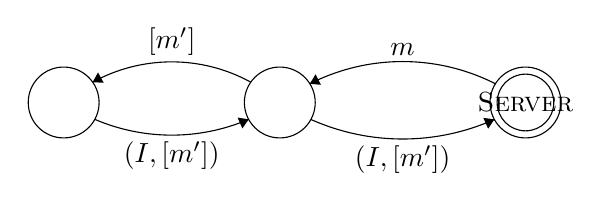
\begin{tikzpicture}[scale=0.15]
\tikzstyle{every node}+=[inner sep=0pt]
\draw [black] (66,-23.1) circle (3);
\draw (66,-23.1) node {\server};
\draw [black] (66,-23.1) circle (2.4);
\draw [black] (45.2,-23.1) circle (3);
\draw (45.2,-23.1) node {\host};
\draw [black] (26.9,-23.1) circle (3);
\draw (26.9,-23.1) node {\user};
\draw [black] (47.743,-21.516) arc (116.95563:63.04437:17.332);
\fill [black] (47.74,-21.52) -- (48.68,-21.6) -- (48.23,-20.71);
\draw (55.6,-19.13) node [above] {$m$};
\draw [black] (29.352,-21.382) arc (118.8302:61.1698:13.89);
\fill [black] (29.35,-21.38) -- (30.29,-21.43) -- (29.81,-20.56);
\draw (36.05,-19.16) node [above] {$[m']$};
\draw [black] (42.565,-24.526) arc (-66.78269:-113.21731:16.527);
\fill [black] (42.57,-24.53) -- (41.63,-24.38) -- (42.03,-25.3);
\draw (36.05,-26.36) node [below] {$(I,[m'])$};
\draw [black] (63.369,-24.535) arc (-65.91058:-114.08942:19.034);
\fill [black] (63.37,-24.53) -- (62.43,-24.4) -- (62.84,-25.32);
\draw (55.6,-26.69) node [below] {$(I,[m'])$};
\end{tikzpicture}
\end{center}
\caption{Finite state machine that depicts the interaction between the user (\user), host (\host) and the server (\server).}
\label{fig:fsm}
\end{figure}

\begin{figure}[h]
\begin{center}
\tikzset{
  every picture/.append style={
    transform shape,
    scale=0.8
  }
 }
\begin{sequencediagram}
\newinst{u}{\user}
\newinst[3]{h}{\host}
\newinst[3]{s}{\server}
\mess{s}{$m$}{h}
\mess{h}{$[m']_1$}{u}
\mess{u}{$I_1,[m']_1$}{h}
%\mess{h}{$[m']_2$}{u}
%\mess{u}{$I_2,[m']_2$}{h}
\mess{h}{...}{u}
\mess{u}{...}{h}
\mess{h}{$[m']_n$}{u}
\mess{u}{$I_n,[m']_n$}{h}
\mess{h}{$I_1,I_2,...,I_n$}{s}
\mess{h}{$[m']_1,[m']_2,...,[m']_n$}{s}
\end{sequencediagram}
\end{center}
\caption{Protocol transcript between the \server, \user and \host that shows one trace from the FSM depicted in Figure~\ref{fig:fsm}.}
\label{fig:protocol}
\end{figure}

\subsection{Interaction Protocol} 

The interaction between the server (\server), user (\user) and host (\host) is depicted in the finite state machine in Figure~\ref{fig:fsm}. \server sends a message $m$ to \host. One can assume $m$ to be the HTML, JS send from \server. We denote $[m]$ to be the render of $m$ by the \host. As \host is malicious, it can transform $m$ to $m'$. Note that the transformation is public knowledge and is deterministic. If $m\neq m'$ then given $[m]$ and $[m']$, \server can determine that $[m]\neq [m']$. We denote the user input to be $I$ which corresponds to a specific $[m]$. 
%Note that the communication channel between \server to \user is neither authenticated, neither confidential. But the communication channel from \user and \server is authenticated. 
In this model, we simplify the user input by assuming that the \user only provides an input $I$ only after observing a message transformation $[m]$. The user provides both her input $I$ and transformation $[m']$ observed by her to \host. The interaction loop between \host and \user can continue until \user finishes her input. After every input \host hands over new message transformation to \user (either result of the input or new message from \server or both). Once the user provides all her inputs, \host send the pairs $(I, [m'])$ to \server.

We also define two functions:
\begin{align*}
\texttt{Input()}&:[m]\rightarrow I \\
\texttt{Transform()}&:m,I\rightarrow [m'],\ \exists i\in I:i=\phi
\end{align*}
Both of them are \emph{bijective}.

One trace of the protocol transcript is depicted in Figure~\ref{fig:protocol}. As described in the FSM, \server receives traces of message transformation ($[m']_1,[m']_2,\ldots,[m']_n$) and corresponding inputs ($I_1,I_2,\ldots,I_n$). From these traces \server could determine of all the $[m']_i$ are in proper form by verifying if $[m]_i=[m']_i$.

\begin{definition}{\textbf{Input integrity}}
\label{def:inputIntegrity}

Assume that \server handed a message $m$ to \host where the proper message transformation is $[m]$. The host changes the message transformation to $[m']$ where $[m']\neq [m]$. We also define correct \user input to be $I$ when \host sends a correct message transformation $[m]$ to \user. We define input integrity as the property where the \server does not accept input $I'$ where $I'\neq I$from \user if the \host changes the message transformation.
\end{definition}

\begin{definition}{\textbf{Output integrity}}
\label{def:outputIntegrity}
Assume that \server handed a message $m$ to \host where the proper message transformation is $[m]$. Output integrity defines that in all circumstances, \user receives the correct message transformation $[m]$ from \host.
\end{definition}

\myparagraph{Verification process} \server checks $\forall i=1\ldots n$ $$[m']_i = \texttt{Transform}(m_{i-1}, I_{i-1})$$ where $I_0=\phi$.

\begin{theorem}
\label{theorem:th1}
If \user does not send all the transformations till $[m']_i$ corresponding to the input $I_i$, input integrity can not be achieved. 
\end{theorem}

\begin{proof}
If \user does not attach all the transformation till $[m']_i$, i.e., $[m']_1, [m']_2, \ldots, [m']_{i-1}, [m']_i$  corresponding to inputs $I_1, I_2,\ldots, I_{i-1}, I_i$, then the server can not verify all the transformations corresponding to the input. \host could modify a specific $[m]_x$ to influence \user input.
\end{proof}

\begin{theorem}
\label{theorem:th2}
If the channel from \user and \server is not authenticated, input integrity is not achievable. But the channel from \server to \user does not require to be secure as long a \user provides the message transformation $[m']_i$ corresponding to every input $I_i$.
\end{theorem}

\begin{proof}
The proof is trivial. If the channel from \user to \server is not authenticated, any input provided by \user can be manipulated by \host without a trace. Hence input integrity is not achievable. As long as \user sends message transformation along with the input, a manipulated message transformation bt \host would be detectable by \server (see Theorem~\ref{theorem:th1}).
\end{proof}

\begin{theorem}
\label{theorem:th3}
Ensuring output integrity also ensures input integrity provided there is an authenticated channel from \user to \server.
\end{theorem}

\begin{proof}
This proof is also trivial. As we describe in the Definition~\ref{def:inputIntegrity} and~\ref{def:outputIntegrity}, if all the message transform from \host $[m']=[m]$, and \host always executes \texttt{transform()} properly, the input integrity is preserved. As \name ensures output integrity and all the input from the user is signed by the \device, \name preserves input integrity. 
\end{proof}




\end{document}
